\section{Versuchsaufbau}
\label{sec:Versuchsaufbau}

Um die Interaktion mit Luftmolekülen möglichst gering zu 
halten, wird eine Hochvakuumdiode verwendet. Diese Diode
ist im wesentlichen ein evakuierter Glaskörper, in dem ein
Draht eingeschmolzen wurde. Dieser Draht wird von Außen 
durch eine Heizspannung erhitzt. Das ist die Glühkathode.
Der Draht besteht aus Wolfram und wird auf Temperaturen
von $1000 \si{\kelvin}$ bis $3000 \si{\kelvin}$ erwärmt.
Die hier durch den glühelektrischen Effekt freiwerdenden 
Elektronen werden durch eine der Kathode gegenüberstehenden
Anode beschleunigt und "abgesaugt". Der beim Auftreffen
auf die Anode entstehende Strom kann mit einem Voltmeter 
gemessen werden.\\
Eine schematische Zeichnung des Hochvakuumdiode ist in 
\autoref{Abb:Diode} zu finden.
\begin{figure}[H]
    \centering
    \caption{Schematische Darstellung der \textit{Hochvakuumdiode}.\cite{sample}}
    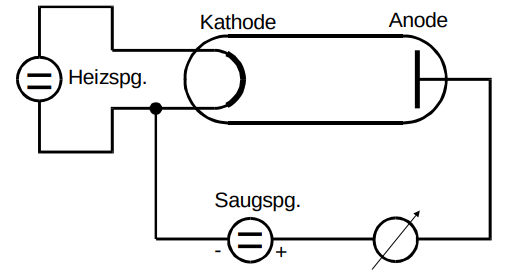
\includegraphics[width=\textwidth]{Bilder/Diode.png}
    \label{Abb:Diode}
\end{figure}

Desweiteren wird für den Versuch ein regelbares Konstantspannungsgerät
und ein Nanoamperemeter benötigt.

\section{Durchführung}
\label{sec:Durchführung}

\subsection{Kennlinienchar einer Hochvakuumdiode}

In diesem Versuchsteil soll eine Kennlinienchar einer 
Hochvakuumdiode aus mindestens 5 Kennlinien erstellt werden 
und daraus der Sättigungsstrom $I_S$ abgelesen werden.
Zudem soll für die maximal mögliche Heizleistung ($2,5 \, \si{\volt}$)
ungefähr der Gültigkeitsbreeich des Langmuir-Schottkyschen
Raumladungsgesetzes gefunden werden und der Exponent der
Strom-Spannungs-Beziehung bestimmt werden.
Der hierfür verwendete Versuchsaufbau ist in \autoref{Abb:Aufbau1}
dargestellt.
\begin{figure}[H]
    \centering
    \caption{Schaltung zur Aufnahme von \textit{Diodenkennlinien}.\cite{sample}}
    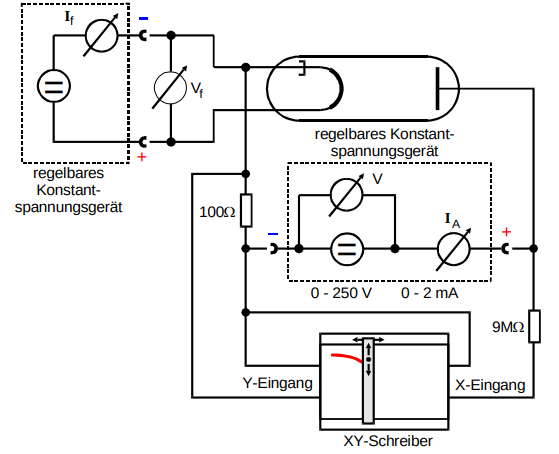
\includegraphics[width=\textwidth]{Bilder/Aufbau1.png}
    \label{Abb:Aufbau1}
\end{figure}
Anstelle des eingezeichneten XY-Scheibers wird jedoch
aus zeitgemäßen Gründen ein Voltmeter verwendet, über das 
auch die Heizspannung eingestellt werden kann. Es werden Insgesamt
5 verschiedene Heizstrom zwischen $1,9$ und $2,5 \, \si{\ampere}$
verwendet und in Abhängigkeit der Beschleunigungsspannung
die Anodenströme notiert. In den 5 gewählten Heizspannung
sollte $2,5 \, \si{\ampere}$ beinhaltet sein, damit
man den Gültigkeitsbreeich des Langmuir-Schottkyschen
Raumladungsgesetzes finden kann.

\subsection{Anlaufstromgebiet der Diode}

Bei diesem Versuch wird die maximal mögliche Heizleistung
von $2,5 \, \si{\ampere}$ verwendet. Der Versuchsaufbau 
wird leicht variiert, da der Anlaufstrom nur sehr gering
ist und mit einem Nanoamperemeter abgelesen werden muss.
Der neue Aufbau ist in \autoref{Abb:Aufbau2} zu sehen.
\begin{figure}[H]
    \centering
    \caption{Schaltung zur Aufnahme des \textit{Anlaufstromgebietes}.\cite{sample}}
    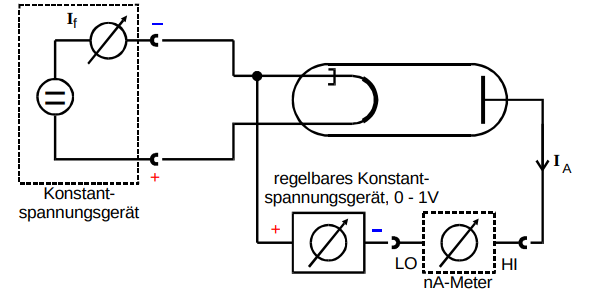
\includegraphics[width=\textwidth]{Bilder/Aufbau2.png}
    \label{Abb:Aufbau2}
\end{figure}
Die Heizspannung wird angelegt und am Nanoamperemeter der fließende
Strom abgelesen.
Es wird mit der Beschleunigungsspannung nach und nach ein
immer höheres Gegenfeld angelegt, bis kein Anodenstrom mehr
messbar ist.